\subsection{Question 1}
\begin{enumerate}
\item Le reseau représentant une sémaphore
\begin{figure}[H]
  \centering
  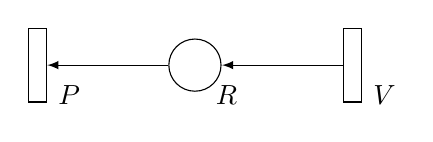
\begin{tikzpicture}
    % Liste des places
    \draw (0,0) node[below right = 4pt] {$R$};
    \node[draw,circle,scale=2] (R) at (0, 0) {};
    
      % Liste des transitions
    \draw (2,0) node[below right= 4pt] {$V$};
    \node[draw,rectangle,yscale=4] (V) at (2, 0) {};
    \draw (-2,0) node[below right= 4pt] {$P$};
    \node[draw,rectangle,yscale=4] (P) at (-2, 0) {};

     % Liste des arcs
    \draw[->,>=latex] (V) -- (R);
    \draw[->,>=latex] (R) -- (P);

  \end{tikzpicture}
  \caption{Réseau de petri associé à la sémaphore} \label{fig:M1}
\end{figure}


\item Simulation de l'évolution du réseau
Lorsqu'une ressource est mise à disposition, on a :

\begin{figure}[H]
  \centering
  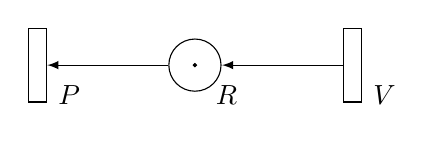
\begin{tikzpicture}
    % Liste des places
    \draw (0,0) node[below right = 4pt] {$R$};
    \node[draw,circle,scale=2] (R) at (0, 0) {};
    
      % Liste des transitions
    \draw (2,0) node[below right= 4pt] {$V$};
    \node[draw,rectangle,yscale=4] (V) at (2, 0) {};
    \draw (-2,0) node[below right= 4pt] {$P$};
    \node[draw,rectangle,yscale=4] (P) at (-2, 0) {};

     % Liste des arcs
    \draw[->,>=latex] (V) -- (R);
    \draw[->,>=latex] (R) -- (P);

     %Marquage
    \draw [fill](0,0) circle (0.02);

  \end{tikzpicture}
  \caption{Réseau de petri associé à la sémaphore} \label{fig:M1}
\end{figure}

On met à disposition une nouvelle ressource: 

\begin{figure}[H]
  \centering
  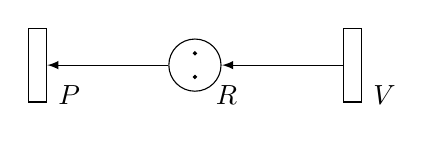
\begin{tikzpicture}
    % Liste des places
    \draw (0,0) node[below right = 4pt] {$R$};
    \node[draw,circle,scale=2] (R) at (0, 0) {};
    
      % Liste des transitions
    \draw (2,0) node[below right= 4pt] {$V$};
    \node[draw,rectangle,yscale=4] (V) at (2, 0) {};
    \draw (-2,0) node[below right= 4pt] {$P$};
    \node[draw,rectangle,yscale=4] (P) at (-2, 0) {};

     % Liste des arcs
    \draw[->,>=latex] (V) -- (R);
    \draw[->,>=latex] (R) -- (P);

     %Marquage
    \draw [fill](0,0.15) circle (0.02);
    \draw [fill](0,-0.15) circle (0.02);

  \end{tikzpicture}
  \caption{Réseau de petri associé à la sémaphore} \label{fig:M1}
\end{figure}

Une ressource est monopolisée, on revient à la fig. 20\\
Et si on monopolise une nouvelle ressource on revient au graphe initial (fig. 19)\\
A ce moment, il est impossible d'acceder à une ressource tant qu'elle n'est pas mise à disposition comme vu précédemment.

\item Transitions concurente?

Dans le cas où le marquage de la place $R$ est non nul, les deux transitions peuvent être franchit indépendement.
Dans le cas ou le marquage de la place $R$ est nul, la transition $V$ peut être franchit, mais pas la transition P.
Cependant, l'incapacité de franchissement de P n'est pas du au franchissement de V.
Donc ces deux transition ne sont pas concurrentes.


\end{enumerate}


